%===============================================================================
% (c) Dominik Harmim <xharmi00@stud.fit.vutbr.cz>
%===============================================================================


\documentclass{ExcelAtFIT}


\usepackage{bm}
\usepackage{amsthm}
\usepackage{wrapfig}
\usepackage[normalem]{ulem}
\usepackage{mathtools}
\usepackage{natbib}
\usepackage{etoolbox}
\usepackage{multirow}

% Solves first/last row of the paragraph on the previous/next page.
\clubpenalty=10000
\widowpenalty=10000

\interfootnotelinepenalty=10000 % do not separate footnotes to multiple pages

% Example theorem.
\newtheoremstyle{example}
    {.2em} % above space
    {.2em} % below space
    {\normalfont} % body font
    {0pt} % indent
    {\bfseries} % head font
    {.} % head punctuation
    {5pt plus 1pt minus 1pt} % head space
    {} % custom head specification
\theoremstyle{example}
\newtheorem{example}{Example}[section]

\renewcommand{\ttdefault}{lmtt} % set Latin Modern tt as tt

% /uv command
\def\uv#1{\iflanguage{british}{``#1''}{\quotedblbase #1\textquotedblleft}}

%%% BEGIN listings settings %%%
\definecolor{bluekeywords}{rgb}{.13, .13, 1}
\definecolor{greencomments}{rgb}{0, .5, 0}
\definecolor{redstrings}{rgb}{.9, 0, 0}
\definecolor{gray}{rgb}{.4, .4, .4}

\lstset{
    basicstyle=\ttfamily,
    backgroundcolor=\color{yellow!10},
    columns=fullflexible,
    showstringspaces=false,
    commentstyle=\color{gray}\upshape,
    captionpos=b,
    tabsize=4,
    keepspaces=true,
    belowskip=-.9\baselineskip,
    aboveskip=.2\baselineskip
}

\lstdefinestyle{c}{
    language=c,
    showspaces=false,
    showtabs=false,
    breaklines=true,
    showstringspaces=true,
    breakatwhitespace=true,
    escapeinside={<@}{@>},
    commentstyle=\color{greencomments},
    keywordstyle=\color{bluekeywords},
    stringstyle=\color{redstrings},
    basicstyle=\ttfamily,
    captionpos=b,
    numbers=left,
    xleftmargin=1.5em,
    frame=trBL
}
%%% END listings settings %%%


%===============================================================================
% REVIEW vs. FINAL VERSION
%===============================================================================
\ExcelFinalCopy


%===============================================================================
% PDF CUSTOMISATION
%===============================================================================
\hypersetup{%
    pdftitle={Advanced Static Analysis of Atomicity in Concurrent Programs through Facebook Infer},
    pdfauthor={Dominik Harmim <xharmi00@stud.fit.vutbr.cz>},
    pdfsubject={Excel@FIT 2021 Paper},
    pdfkeywords={Facebook Infer, Static Analysis, Abstract Interpretation, Atomicity Violation, Contracts for Concurrency, Concurrent Programs, Program Analysis, Atomicity, Atomer}%
}


%===============================================================================
% ARTICLE INFORMATION
%===============================================================================
\ExcelYear{2021}

\PaperTitle{Advanced Static Analysis of Atomicity in Concurrent Programs through Facebook Infer}

\Authors{Dominik Harmim*}
\affiliation{%
    *\href{mailto:xharmi00@stud.fit.vutbr.cz}{xharmi00@stud.fit.vutbr.cz},
    \textit{Faculty of Information Technology, Brno University of Technology}%
}

\Keywords{Facebook Infer\,---\,Static Analysis\,---\,Abstract Interpretation\,---\,Atomicity Violation\,---\,Contracts for Concurrency\,---\,Concurrent Programs\,---\,Program Analysis\,---\,Atomicity\,---\,Atomer}

\Supplementary{%
    \href{https://github.com/harmim/infer}{Atomer Repository}%
    \,---\,\href{https://github.com/harmim/infer/wiki}{Atomer Wiki}%
    \,---\,\href{https://github.com/facebook/infer}{Facebook Infer Repository}%
}


%===============================================================================
% ABSTRACT and TEASER
%===============================================================================

\Abstract{%
    \emph{Atomer} is a~\emph{static analyser} based on the idea that if some \emph{sequences of functions} of a~\emph{multi-threaded program} are executed \emph{under locks} in some runs, likely, they are \emph{always intended to execute atomically}. Atomer thus strives to look for such sequences and then detects for which of them the atomicity may be broken in some other program runs. The first version of Atomer was proposed within the BSc thesis of the author of this paper and implemented as a~plugin of the \emph{Facebook Infer framework}. In this paper, a~new and \emph{significantly improved} version of Atomer is proposed. The improvements aim at both increasing \emph{scalability} as well as \emph{precision}. Moreover, support for several initially not supported programming features has been added (including, e.g., the possibility of analysing \emph{C++ and Java programs} or support for \emph{re-entrant locks} or \emph{lock guards}). Through a~number of experiments (including experiments with \emph{real-life code} and \emph{real-life bugs}), it is shown that the new version of Atomer is indeed much more \emph{general}, \emph{scalable}, and \emph{precise}.%
}

\Teaser{\TeaserImage{teaser.pdf}}


%===============================================================================
\begin{document}


% spacing around math mode
\setlength{\abovedisplayskip}{.3em}
\setlength{\belowdisplayskip}{.3em}

% spacing before footnote
\addtolength{\skip\footins}{-.3em}


\startdocument


%===============================================================================
% ARTICLE CONTENTS
%===============================================================================


%===============================================================================
\section{Introduction}

Bugs have been present in computer programs ever since the inception of the programming discipline. Unfortunately, they are often hidden in unexpected places, and they can lead to unexpected behaviour, which may cause significant damage. Nowadays, developers have many possibilities of catching bugs in the early development process. \emph{Dynamic analysers} or tools for \emph{automated testing} are often used, and they are satisfactory in many cases. Nevertheless, they can still leave too many bugs undetected because they can analyse only \emph{particular program flows} dependent on the input data. An alternative solution is \emph{static analysis} (despite it, of course, suffers from some problems too\,---\,such as the possibility of reporting many \emph{false alarms}\footnote{So-called \textbf{false alarms} (also \emph{false positives}) are incorrectly reported errors, i.e., actually, they are not errors.}). Quite some tools for static analysis were implemented, e.g., Coverity or CodeSonar. However, they are often proprietary and difficult to openly evaluate and extend.

Recently, Facebook introduced \emph{Facebook Infer}: an \emph{open-source} tool for creating \emph{highly scalable}, \emph{compositional}, \emph{incremental}, and \emph{interprocedural} static analysers. Facebook Infer has grown considerably, but it is still under active development. It is employed every day not only in Facebook itself but also in other companies, such as Spotify, Uber, Mozilla, or Amazon. Currently, Facebook Infer provides several analysers that check for various types of bugs, such as buffer overflows, data races and some forms of deadlocks and starvation, null-dereferencing, or memory leaks. However, most importantly, Facebook Infer is a~\emph{framework} for building new analysers quickly and easily. Unfortunately, the current version of Facebook Infer still lacks better support for \emph{concurrency bugs}. While it provides a~reasonably advanced data race analyser, it is limited to Java and C++ programs only and fails for C~programs, which use a~\emph{lower-level lock manipulation}. Moreover, the only available checker of \emph{atomicity of call sequences} is the first version of \emph{Atomer}~\cite{harmimBP} proposed in the bachelor's thesis of the author.

At the same time, in \emph{concurrent programs}, there are often \emph{atomicity requirements} for the execution of specific sequences of instructions. Violating these requirements may cause many kinds of problems, such as unexpected behaviour, exceptions, segmentation faults, or other failures. \emph{Atomicity violations} are usually not verified by compilers, unlike syntactic or some sorts of semantic rules. Moreover, atomicity requirements, in most cases, are not even documented at all. Therefore, in the end, programmers themselves must abide by these requirements and usually lack any tool support. Furthermore, in general, it is difficult to avoid errors in \emph{atomicity-dependent programs}, especially in large projects, and even more laborious and time-consuming is finding and fixing them. The paper~\cite{contracts2017} discusses the importance of \emph{atomicity-related bugs}, and it also shows some bugs in \emph{real-world programs}. Unfortunately, tool support for automatically discovering such kinds of errors is currently minimal.

As already mentioned, within the author's bachelor's thesis~\cite{harmimBP}, \emph{Atomer}\footnote{The implementation of~\textbf{Atomer} is available at GitHub. The link can be found among the supplementary materials of this paper.} was proposed\,---\,a~\emph{static analyser} for finding some forms of \emph{atomicity violations} implemented as a~Facebook Infer's module. In particular, the stress is put on the \emph{atomic execution of sequences of function calls}, which is often required, e.g., when using specific library calls. For example, assume the function from Listing~\ref{list:exampleViolation} that replaces item~\texttt{a} in an array by item~\texttt{b}. It contains atomicity violation\,---\,the index obtained may be outdated when \texttt{set} is executed, i.e., \texttt{index\_of} and \texttt{set} should be executed atomically. The analysis is based on the assumption that sequences of function calls executed \emph{atomically once} should probably be executed \emph{always atomically}. Hence, the checker naturally works with sequences. In fact, the idea of checking the atomicity of certain sequences of function calls is inspired by the work of \emph{contracts for concurrency}~\cite{contracts2017}. In the terminology of~\cite{contracts2017}, the atomicity of specific sequences of calls is the most straightforward (yet very useful in practice) kind of contracts for concurrency. However, while the idea of using sequences in the given context is indeed natural and rather exact, it quite severely limits the \emph{scalability} of the analysis (indeed, even with a~few functions, there can appear numerous different orders in which they can be called). Moreover, the implementation of the first version of Atomer targets mainly \emph{C~programs} using \emph{PThread locks}. Consequently, there was no support for other languages and their locking mechanisms in the first version of Atomer.

\begin{lstlisting}[
    style=c, label={list:exampleViolation}, float=hbt,
    caption={Example of \emph{atomicity violation}}
]
void replace(int a, int b) {
    int i = array.index_of(a);
    if (i >= 0) array.set(i, b); }
\end{lstlisting}

Within this work, Atomer has been significantly improved and extended. In particular, to improve scalability, working with sequences of function calls was \emph{approximated} by working with \emph{sets of function calls}. Furthermore, several new features were implemented: support for \emph{C++ and Java}, including various advanced kinds of locks these languages offer (such as \emph{re-entrant locks} or \emph{lock guards}); or a~more precise way of \emph{distinguishing between different lock instances}. Moreover, the analysis has been \emph{parameterised} by function names to concentrate on during the analysis and limits of the number of functions in \emph{critical sections}. These parameters aim to reduce the number of false alarms. Their proposal is based on the author's analysis of false alarms produced by the first Atomer's version. Lastly, new experiments were performed to test capabilities of the new version of Atomer.

The development of the original Atomer started under the H2020 ECSEL projects AQUAS and Arrowhead Tools. The development of its new version is supported by the H2020 ECSEL project VALU3S. The development has been discussed with the developers of Facebook Infer too. Parts of the paper concerning the Facebook Infer framework and the basic version of Atomer are partially taken from the thesis~\cite{harmimBP}.

The rest of the article is organised as follows. In Section~\ref{sec:infer}, there is introduced the \emph{Facebook Infer} framework. The original version of \emph{Atomer} and related work are described in Section~\ref{sec:atomer}. Subsequently, Section~\ref{sec:proposal} presents all the proposed extensions and improvements. The implementation of these extensions, together with the experimental evaluation of the new Atomer's features and other experiments performed within this work, are discussed in Section~\ref{sec:exp}. Finally, the paper is concluded in Section~\ref{sec:conc}.


%===============================================================================
\section{Facebook Infer}
\label{sec:infer}

This section describes the principles and features of \emph{Facebook Infer}. The description is based on information provided at the Facebook Infer's website\footnote{\textbf{Facebook Infer's} website: \url{https://fbinfer.com}.}. Parts of this section are taken from~\cite{harmimBP}.

Facebook Infer is an \emph{open-source}\footnote{A~link to the \textbf{Facebook Infer's open-source repository} is in the supplementary materials of the paper.} \emph{static analysis framework}, which can discover various kinds of software bugs and which stress the \emph{scalability} of the analysis. For an explanation of the general meaning of static analysis, see, e.g., \cite{staticAnalysisMoller, programAnalysisNielson, staticAnalysisRival}. A~more detailed explanation of Facebook Infer architecture is given in Section~\ref{sec:fbinferArch}. Facebook Infer is implemented in \emph{OCaml}\,---\,a~\emph{functional} programming language, also supporting \emph{imperative} and \emph{object-oriented} paradigms. Infer has initially been a~rather specialised tool focused on \emph{sound verification} of the absence of \emph{memory safety violations}, which was first published in the well-known paper~\cite{inferBiabduction}. Once Facebook has purchased it, its scope significantly widened and abandoned the focus on sound analysis only.

Facebook Infer can analyse programs written in the following languages: C, C++, Java, Obj-C, C\#. Moreover, it is possible to extend Facebook Infer's \emph{frontend} for supporting other languages. Currently, Infer contains many analyses focusing on various kinds of bugs, e.g., \emph{Inferbo} (buffer overruns); \emph{RacerD} (data races)~\cite{racerD}; and other analyses that check for buffer overflows, some forms of deadlocks and starvation, null-dereferencing, memory leaks, resource leaks, etc.

\subsection{Abstract Interpretation in Facebook Infer}

Facebook Infer is a~general framework for static analysis of programs, and it is based on \emph{abstract interpretation}, which is explained in~\cite{AILatticeModelCousot, staticAnalysisMoller, programAnalysisNielson, staticAnalysisRival}. Despite the original approach taken from~\cite{inferBiabduction}, Facebook Infer aims to find bugs rather than perform \emph{formal verification}. It can be used to quickly develop new sorts of \emph{compositional} and \emph{incremental} analysers (both \emph{intraprocedural} and \emph{interprocedural}~\cite{programAnalysisNielson}) based on the concept of function \emph{summaries}. In general, a~\emph{summary} represents \emph{preconditions} and \emph{postconditions} of a~function~\cite{hoare}. However, in practice, a~summary is a~custom data structure that may be used for storing any information resulting from the analysis of particular functions. Facebook Infer generally does not compute the summaries during the analysis along the \emph{Control Flow Graph} (\textbf{CFG}~\cite{controlFlowAnalysisAllen}) as it is done in classical analyses based on the concepts from~\cite{DFAGraphReach, DFAApproaches}. Instead, Facebook Infer performs the analysis of a~program \emph{function-by-function along the call tree}, starting from its leaves. Therefore, a~function is analysed, and a~summary is computed without knowledge of the call context. Then, the summary of a~function is used at all of its call sites. Since the summaries do not differ for different contexts, the analysis becomes more scalable, but it can lead to a~loss of accuracy.

In order to create a~new intraprocedural analyser in Facebook Infer, it is needed to define the following (the listed items are described in more detail in~\cite{harmimBP}):
\begin{enuminline}
    \item The \emph{abstract domain}~$ \boldsymbol{Q} $, i.e., the type of \emph{abstract states};

    \item The \emph{ordering operator}~$ \sqsubseteq $, i.e., an ordering of abstract states;

    \item The \emph{join} operator~$ \sqcup $, i.e., the way of joining two abstract states;

    \item The \emph{widening} operator~$ \triangledown $, i.e., the way how to enforce termination of the computation;

    \item And the \emph{transfer functions}~$ \tau $, i.e., transformers that take an abstract state as an input and produce an abstract state as an output.
\end{enuminline}
Further, to create an interprocedural analyser, it is required to define additionally:
\begin{enuminline}
    \item The type of function summaries~$ \chi $.

    \item The logic for using summaries in transfer functions and the logic for transforming an intraprocedural abstract state to a~summary.
\end{enuminline}

An important Infer's feature, which improves its scalability, is the \emph{incrementality} of the analysis. It allows one to analyse separate code changes only, instead of analysing the whole codebase. It is more suitable for extensive and variable projects where ordinary analysis is not feasible. The incrementality is based on \emph{reusing summaries} of functions for which there is no change in them neither in the functions transitively invoked from them, as shown in Example~\ref{ex:inferAnalysis}.

\subsection{Architecture of the Infer AI}
\label{sec:fbinferArch}

The architecture of the abstract interpretation framework of Infer (\textbf{Infer AI}) may be split into three major parts: the \emph{frontend}, an \emph{analysis scheduler} (and the \emph{results database}), and a~set of \emph{analyser plugins}.

The frontend compiles input programs into the \emph{Smallfoot Intermediate Language} (SIL) and represents them as a~CFG. There is a~separate CFG representation for each analysed function. Nodes of this CFG are formed as SIL instructions (the individual instructions are outlined in~\cite{harmimBP}). The frontend allows one to propose \emph{language-independent} analyses (to a~certain extent) because it supports input programs to be written in multiple languages.

The next part of the architecture is the scheduler, which defines the order of the analysis of single functions according to the appropriate \emph{call graph}\footnote{\textbf{A~call graph} is a~\emph{directed graph} describing call dependencies among functions.}. The scheduler also checks if it is possible to simultaneously analyse some functions, allowing Facebook Infer to run the analysis in parallel.

\clearpage

\begin{example}
    \label{ex:inferAnalysis}
\end{example}
\vspace{-.3em}
\noindent
\begin{wrapfigure}{r}{.42 \linewidth}
    \centering
    \vspace{-1em}
    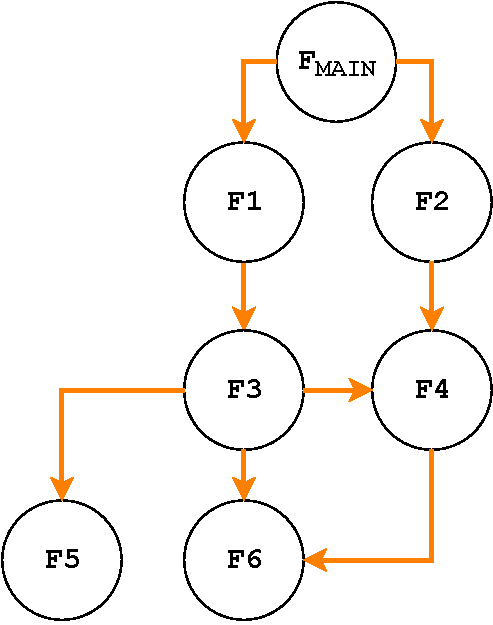
\includegraphics[width=.2 \textwidth]{infer-call-graph.pdf}
    \captionof{figure}{A~call graph for an illustration of Facebook Infer's analysis process~\cite{harmimBP}}
    \label{fig:inferCallGraph}
\end{wrapfigure}
For demonstrating the order of the analysis in Facebook Infer and its incrementality, assume the call graph given in Figure~\ref{fig:inferCallGraph}. At first, leaf functions \texttt{F5} and \texttt{F6} are analysed. Further, the analysis goes on towards the root of the call graph\,---\,\texttt{F\textsubscript{MAIN}}, while considering the dependencies denoted by the edges. This order ensures that a~summary is available once a~nested function call is abstractly interpreted within the analysis. When there is a~subsequent code change, only directly changed functions and all the functions up the call path are re-analysed. For instance, if there is a~change of source code of function \texttt{F4}, Facebook Infer triggers reanalysis of functions \texttt{F4}, \texttt{F2}, and \texttt{F\textsubscript{MAIN}} only.

The last part of the architecture consists of analyser plugins. Each plugin performs some analysis by interpreting SIL instructions. The result of the analysis of each function (function summary) is stored in the results database. The interpretation of SIL instructions (\emph{commands}) is made using the \emph{abstract interpreter} (also called the \emph{control interpreter}) and \emph{transfer functions} (also called the \emph{command interpreter}). The transfer functions take a~previously generated \emph{abstract state} of an analysed function as an input, and by applying the interpreting command, produce a~new abstract state. The abstract interpreter interprets the command in an \emph{abstract domain} according to the CFG.


%===============================================================================
\section{\hspace{-.15em}Atomer: Atomicity Violations Detector}
\label{sec:atomer}

This section introduces the principles of the basic version of the \emph{Atomer static analyser} for finding some forms of \emph{atomicity violations} proposed in the bachelor's thesis~\cite{harmimBP} of the author of this paper. Therefore, naturally, the following description is based on the mentioned thesis.

\subsection{Related Work}

Atomer is slightly inspired by ideas from~\cite{contracts2017}. In that paper, there is described a~proposal and implementation of a~\emph{static} approach for finding \emph{atomicity violations of sequences of function calls}, which is based on \emph{grammars} and \emph{parsing trees}. Note that in the paper~\cite{contracts2017}, there is also described and implemented a~\emph{dynamic} approach for the validation. The authors of the paper implemented a~stand-alone prototype static analyser called \emph{Gluon} for analysing programs written in Java. To the best author's knowledge, Gluon is the only static analyser that tries to go in a~similar direction as Atomer does. Gluon led to some promising experimental results, but the \emph{scalability} of the tool was still limited. Moreover, Gluon is no more developed, and it is not easy to use. Despite all author's efforts, it was not put into operation. Above that, the authors themselves note that the code of Gluon is very ad hoc, and many things are hard-coded in it. These facts, in fact, inspired the decision that eventually led to the implementation of Atomer, namely, to get inspired by the ideas from~\cite{contracts2017}, but reimplement them in \emph{Facebook Infer}, redesigning it following the principles of Facebook Infer, which should make the resulting tool more scalable. In the end, however, due to adapting the analysis to the context of Facebook Infer, the implementation of Atomer's analysis is significantly different from~\cite{contracts2017}. Furthermore, unlike Gluon, the new version of Atomer is capable of analysing a~much wider range of programs because it also supports other languages than Java, and it supports more advanced locking mechanisms. On the other hand, Gluon also implements \emph{extended contracts for concurrency}~\cite{contracts2017} that consider \emph{data flow} within functions and \emph{contextual information}. These should improve the precision of the analysis. It is author's future work to implement these extended contracts in Atomer as well.

\subsection{Analysis and Design}

Atomer concentrates on checking the \emph{atomicity of the execution of certain sequences of function calls}, which is often required for \emph{concurrent programs'} correct behaviour. In principle, Atomer is based on the assumption that sequences of function calls executed \emph{atomically once} should probably be executed \emph{always atomically}. Atomer can both automatically derive those sequences that are sometimes executed atomically as well as subsequently check whether they are always executed atomically. Both of these steps are done statically. The proposed analysis is thus divided into two parts (\emph{phases of the analysis} that are in-depth described in the sections below):
\begin{enumerate}[label={\textbf{Phase~\arabic*}:}, leftmargin=4.2em]
    \item Detection of (likely) \emph{atomic sequences}.

    \item Detection of \emph{atomicity violations} (violations of the atomic sequences).
\end{enumerate}

This section provides a~high-level view of the \emph{abstract interpretation} underlying Atomer. The abstract states~$ s \in \boldsymbol{Q} $ of both phases of the analysis are proposed as \emph{sets}. So, in fact, the \emph{ordering operator}~$ \sqsubseteq $ is implemented using testing for a~\emph{subset} (i.e., $ s \sqsubseteq s^\prime \Leftrightarrow s \subseteq s^\prime $, where $ s, s^\prime \in \boldsymbol{Q} $), the \emph{join operator}~$ \sqcup $ is implemented as the \emph{set union} (i.e., $ s \sqcup s^\prime \Leftrightarrow s \cup s^\prime $), and the \emph{widening operator}~$ \triangledown $ is implemented using the join operator (i.e., $ s \triangledown s^\prime \Leftrightarrow s \sqcup s^\prime $) since the domains are \emph{finite}.

\subsubsection{Phase~1: Detection of Atomic Sequences}

\textbf{Phase~1} of Atomer detects \emph{sequences of functions} that should be \emph{executed atomically}. It is based on looking for sequences executed atomically, in particular, under some lock, on some path through a~program.

The detection of such sequences is based on analysing all paths through the CFG of a~function and generating all pairs $ {(A, B)} \in {\Sigma^* \times \Sigma^*} $ (where~$ \Sigma $ is the set of functions of a~given program) of \emph{reduced sequences}\footnote{A~\textbf{reduced sequence} denotes a~sequence in which the first appearance of each function is recorded only.} of function calls for each path such that: $ A $~is a~reduced sequence of function calls that appear between the beginning of the function being analysed and the first lock; between an unlock and a~subsequent lock; or between an unlock and the end of the function being analysed. $ B $ is a~reduced sequence of function calls that follow the calls from~$ A $ and that appear between a~lock and an unlock (or between a~lock and the end of the function being analysed). Thus, the \emph{abstract states} of the analysis are elements of the set $ 2^{2^{\Sigma^* \times \Sigma^*}} $ because there is a~set of the ${ (A, B) }$ pairs for each program path.

A~\emph{summary}~$ \chi_\mathtt{f} \in 2^{\Sigma^*} \times \Sigma^* $ of a~function~\texttt{f} is then a~pair $ \chi_\mathtt{f} = (\boldsymbol{B}, AB) $, where:
\begin{itemize}
    \item $ \boldsymbol{B} $ is a~set constructed such that it contains all the~$ B $ sequences that appear on program paths through~\texttt{f}, i.e., those computed within the ${ (A, B) }$ pairs at the exit of~\texttt{f}. In other words, this component of the summary is a~set of sequences of atomic function calls appearing in~\texttt{f}.

    \item $ AB $ is a~\emph{concatenation} of all the~$ A $ and~$ B $ sequences with removed duplicates of function calls. In particular, assume that the following set of ${ (A, B) }$ pairs is computed at the exit of~\texttt{f}: $ \{{(A_1, B_1)}, {(A_2, B_2)}, \ldots, {(A_n, B_n)}\} $, then the result is the sequence $ A_1 \cdot B_1 \cdot A_2 \cdot B_2 \cdot \ldots \cdot A_n \cdot B_n $ with removed duplicates. Intuitively, in this component of the summary, the analysis gathers occurrences of all called functions within the analysed function. $ AB $ are recorded to facilitate the derivation of atomic call sequences that show up higher in the \emph{call hierarchy}. Indeed, while locks/unlocks can appear in such a~\emph{higher-level} function, parts of the call sequences can appear lower in the call hierarchy.
\end{itemize}

\begin{example}
    For instance, the analysis of the function~\texttt{f} from Listing~\ref{list:atomerPhase1} produces the following sequences:
    $$
        \overbrace{\mathtt{x} \cdot \text{\texttt{\sout{x}}} \cdot \mathtt{y}}^A \overbrace{[\mathtt{a} \cdot \mathtt{b} \cdot \text{\texttt{\sout{b}}}]}^B
    $$
    The strikethrough of the functions~\texttt{x} and~\texttt{b} denotes removing already recorded function calls in the~$ A $ and~$ B $ sequences to get the reduced form. For the above, the abstract state at the end of the abstract interpretation of the function~\texttt{f} is $ s_\mathtt{f} = \{\{(\mathtt{x} \cdot \mathtt{y}, \mathtt{a} \cdot \mathtt{b})\}\} $. The derived summary~$ \chi_\mathtt{f} $ for the function~\texttt{f} is $ \chi_\mathtt{f} = {(\{{\mathtt{a} \cdot \mathtt{b}}\}, {\mathtt{x} \cdot \mathtt{y} \cdot \mathtt{a} \cdot \mathtt{b}})} $.
\end{example}

\begin{lstlisting}[
    style=c, label={list:atomerPhase1}, float=hbt,
    caption={A~code snippet used for an illustration of the derivation of \emph{sequences of functions called atomically}}
]
void f() {
    x(); x(); y();
    <@\textcolor{red}{lock}@>(&L); // a.b
    a(); b(); b();
    <@\textcolor{red}{unlock}@>(&L); }
\end{lstlisting}

The derived sequences of calls assumed to execute atomically\,---\,the~$ \boldsymbol{B} $ sequences\,---\,from the summaries of all analysed functions are stored into a~file used during \textbf{Phase~2}, which is described below.

\subsubsection{Phase~2: Detection of Atomicity Violations}

In the second phase of the analysis, i.e., when \emph{detecting violations} of the atomic sequences obtained from \textbf{Phase~1}, the analysis looks for \emph{pairs of functions} that \emph{should be called atomically} (or just for single functions if there is only one function call in an atomic sequence) and that are not executed atomically (i.e., under a~lock) on some path through the CFG. The pairs of function calls to be checked for atomicity are obtained as follows: For each function~\texttt{f} with a~\emph{summary}~$ \chi_\mathtt{f} = {(\boldsymbol{B}, AB)} $ in a~given program, where $ \boldsymbol{B} = {\{B_1, B_2, \ldots, B_n\}} $, the analysis considers \emph{every pair} $ {(\mathtt{x}, \mathtt{y})} \in \Sigma \times \Sigma $ of functions that appear as a~\emph{substring} in some of the~$ B_i $ sequences, i.e., $ B_i = w \cdot \mathtt{x} \cdot \mathtt{y} \cdot w^\prime $ for some sequences~$ w, w^\prime $. Note that~\texttt{x} could be~$ \varepsilon $ (an empty sequence) if some~$ B_i $ consists of a~single function. All these \uv{atomic pairs} are put into the set $ \Omega \in 2^{\Sigma \times \Sigma} $.

An element of this phase's \emph{abstract state} is a~triple $ {(\mathtt{x}, \mathtt{y}, \Delta)} \in \Sigma \times \Sigma \times 2^{\Sigma \times \Sigma} $ where $ {(\mathtt{x}, \mathtt{y})} $ is a~pair of the most recent calls of functions performed on the program path being explored, and~$ \Delta $ is a~set of so far detected \emph{pairs that violate atomicity}. Thus, the abstract states are elements of the set $ 2^{\Sigma \times \Sigma \times 2^{\Sigma \times \Sigma}} $. Whenever a~function~\texttt{f} is called on some path that led to an abstract state ${ (\mathtt{x}, \mathtt{y}, \Delta) }$, a~new pair ${ (\mathtt{x}^\prime, \mathtt{y}^\prime) }$ of the most recent function calls is created from the previous pair ${ (\mathtt{x}, \mathtt{y}) }$ such that $ {(\mathtt{x}^\prime, \mathtt{y}^\prime)} = {(\mathtt{y}, \mathtt{f})} $. Further, when the current program state is not inside an \emph{atomic block}, the analysis checks whether the new pair (or just the last call) violates the atomicity (i.e., $ {(\mathtt{x}^\prime, \mathtt{y}^\prime)} \in \Omega \vee {(\varepsilon, \mathtt{y}^\prime)} \in \Omega $). When it does, it is added to the set~$ \Delta $ of pairs that violate atomicity.

\begin{example}
    \sloppy
    To demonstrate the detection of an atomicity violation, assume the functions~\texttt{f} and~\texttt{g} from Listing~\ref{list:atomerPhase2}. The set of atomic sequences of the function~\texttt{f} with the summary~$ \chi_\mathtt{f} = (\boldsymbol{B}, AB) $ is $ \boldsymbol{B} = \{\mathtt{a} \cdot \mathtt{b} \cdot \mathtt{c}\} $, thus $ \Omega = \{{(\mathtt{a, b})}, {(\mathtt{b, c})}\} $. In the function~\texttt{g}, an atomicity violation is detected because the pair of functions~\texttt{b} and~\texttt{c} is not called atomically.
\end{example}

\begin{lstlisting}[
    style=c, label={list:atomerPhase2}, float=t,
    caption={Example of an \emph{atomicity violation}}
]
void f() {
    <@\textcolor{red}{lock}@>(&L); // a.b.c
    a(); b(); c();
    <@\textcolor{red}{unlock}@>(&L); }
void g() {
    // <@\textcolor{red}{ATOMICITY\_VIOLATION:}@> (b, c)
    x(); b(); c(); y(); }
\end{lstlisting}

The sets of atomicity violations~$ \Delta $ from individual functions are the final reported atomicity violations seen by a~user.


%===============================================================================
\section{\hspace{-.15em}Proposal of Enhancements for Atomer}
\label{sec:proposal}

The above proposal was implemented in the first version of Atomer~\cite{harmimBP}. The implementation works and can be used in practice to analyse various kinds of programs, and it may find \emph{real atomicity-related bugs}. Nevertheless, there are still several limitations and cases where the original version of Atomer would not work correctly, i.e., cases not addressed during the original proposal. Below, the author proposes solutions for some of the limitations. The solutions enhance the analysis's \emph{precision} and \emph{scalability}. Furthermore, Section~\ref{sec:exp} provides an overview of the implementation of a~new version of Atomer.

\subsection{Approximation of Sequences by Sets}

Regarding \emph{scalability}, the basic version of Atomer can have problems with more \emph{extensive} and \emph{complex} programs, which can manifest both in its \emph{time} and \emph{memory} consumption. The problems arise primarily due to working with the sets of ${ (A, B) }$ pairs of \emph{sequences} of function calls in \emph{abstract states} (during \textbf{Phase~1}). It may be necessary to store many of these sequences, and they could be very long (due to all different paths through the CFG of an analysed program). The author's idea is to \emph{approximate} these sets by working with sets of ${ (A, B) }$ pairs of \textbf{sets} of function calls. Apart from representing abstract states of the first phase of the analysis, elements of these pairs do also appear in the first phase's \emph{summaries}, and they are then used during \textbf{Phase~2} as well. Thus, it is needed to make a~certain approximation in the summaries and their subsequent usage too.

In particular, the proposed solution is more scalable because the ordering of function calls that appear in the pairs is not relevant anymore. Therefore, less memory is required because different sequences of function calls can map the same set. The analysis is also faster since there are stored fewer sets of function calls to work with. On the other hand, the analysis is less accurate because the new approach causes some loss of information. In practice, this loss of information could eventually lead to \emph{false alarms}. However, the number of such false alarms is typically not that high as this project's experimental evidence shows.

The \emph{detection of sequences of calls to be executed atomically} now generates all ${ (A, B) }$ pairs of \textbf{sets} of function calls for each path instead of pairs of sequences, i.e., $ {(A, B)} \in 2^\Sigma \times 2^\Sigma $. The purpose of the pairs is preserved. So, the \emph{abstract states} are elements of the set $ 2^{2^{2^\Sigma \times 2^\Sigma}} $. In all the implemented algorithms and definitions, it is sufficient to work with:
\begin{enuminline}
    \item \emph{sets}~$ 2^\Sigma $ of functions, instead of \emph{sequences}~$ \Sigma^* $ of functions;

    \item the \emph{empty set}~$ \emptyset $, instead of the \emph{empty sequence}~$ \varepsilon $;

    \item and \emph{unions}~$ \cup $ of sets, instead of the \emph{concatenation}~$ \cdot $ of sequences.
\end{enuminline}
Consequently, also the form of summaries~$ \chi $ changes from $ 2^{\Sigma^*} \times \Sigma^* $ to $ 2^{2^\Sigma} \times 2^\Sigma $.

\begin{example}
    For demonstrating the approximation of the analysis to sets, assume functions~\texttt{f} and~\texttt{g} from Listing~\ref{list:atomerPhase1Sets}. After the approximation, the produced abstract states and summaries are as follows: $ s_\mathtt{f} = s_\mathtt{g} = \{\{({\{\mathtt{a}, \mathtt{b}\}}, {\{\mathtt{x}, \mathtt{y}\}})\}\} $, $ \chi_\mathtt{f} = \chi_\mathtt{g} = ({\{\{\mathtt{x}, \mathtt{y}\}\}}, \{\mathtt{a}, \mathtt{b}, \allowbreak \mathtt{x}, \mathtt{y}\}) $. This is, they are the same for both functions because there are the same locked/unlocked function calls, only the order of calls differs.
\end{example}

\begin{lstlisting}[
    style=c, label={list:atomerPhase1Sets}, float=hbt,
    caption={A~code snippet used to illustrate the proposed \emph{approximation} of the first phase of the analysis in the new version of Atomer by using \emph{sets of function calls}}
]
void f() {
    a(); b();
    <@\textcolor{red}{lock}@>(&L); // x.y -> {x, y}
    x(); y();
    <@\textcolor{red}{unlock}@>(&L); }
void g() {
    b(); a();
    <@\textcolor{red}{lock}@>(&L); // y.x -> {x, y}
    y(); x();
    <@\textcolor{red}{unlock}@>(&L); }
\end{lstlisting}

\emph{Detection of atomicity violation} in \textbf{Phase~2} then works almost the same way as before the approximation. There is only one difference. Before, the analysis implemented in the second phase looked for violations of atomic sequences obtained from \textbf{Phase~1}. Now, \textbf{atomic sets} are obtained from \textbf{Phase~1}; hence, the detection of atomicity violations needs to work with sets too. The second phase of the analysis now looks for non-atomic execution of any pair of functions~\texttt{f,~g} such that ${ \{\mathtt{f, g}\} }$ is a~\emph{subset} of some set of functions that were found to be executed atomically.

\begin{example}
    \sloppy
    For example, assume that \textbf{Phase~1} analysed a~function~\texttt{f}, which produced the summary $ \chi_f = {(\boldsymbol{B}, AB)} $. Assume that the set~$ \boldsymbol{B} $ of sets of functions that should be called atomically is the following: $ \boldsymbol{B} = \{{\{\mathtt{a}, \mathtt{b}, \mathtt{c}\}}\} $, the analysis now looks for the following pairs of functions that are not called atomically (all 2-element variations): $ \Omega = \{{(\mathtt{a}, \mathtt{b})}, {(\mathtt{a}, \mathtt{c})}, {(\mathtt{b}, \mathtt{a})}, {(\mathtt{b}, \mathtt{c})}, {(\mathtt{c}, \mathtt{a})}, {(\mathtt{c}, \mathtt{b})}\} $.
\end{example}

\subsection{Advanced Manipulation with Locks}

The original version of Atomer does not distinguish \emph{different lock instances} in a~program. Only calls of locks/unlocks are identified, and the parameters of these calls (\emph{lock objects}) are not considered. Thus, if there are several lock objects used, the analysis does not work correctly.

In order to consider lock objects, it was proposed to distinguish between them using Facebook Infer's built-in mechanism called \emph{access paths}~\cite{accessPath}. The analyser does not perform a~classic \emph{alias analysis}, i.e., it does not perform a~precise analysis for saying when arbitrary pairs of accesses to lock objects may alias (such an analysis is considered too expensive).

The \emph{syntactic access paths} represent \emph{heap locations} via the paths used to access them, i.e., they have the form of an expression consisting of a~base variable followed by a~sequence of fields. More formally, let $ Var $ be a~set of all variables that can occur in a~given program. Let $ Field $ be a~set of all possible field names that can be used in the program (e.g., structure fields). An access path~$ \pi $ from the set~$ \Pi $ of all access paths is then defined as follows: $ \pi \in \Pi \Coloneqq Var \times Field^* $. Access paths are already implemented in Facebook Infer. For instance, the principle of using access paths is used in an existing analyser in Facebook Infer\,---\,RacerD~\cite{racerD}\,---\,for data race detection. In general, no sufficiently precise \emph{alias analysis} works \emph{compositionally} and at \emph{scale}. That is the motivation for using access paths in Facebook Infer and Atomer.

During the analysis (both phases), each atomic section is identified by an access path of the lock that guards the section. Because \emph{syntactically identical access paths} are used as the means for distinguishing atomic sections, some atomicity violations could be missed (or some false alarms could be reported) due to distinct access paths that refer to the same memory. However, the analysis's precision is still significantly improved this way while preserving its \emph{scalability}, and the stress is anyway put on finding likely violations, not on being \emph{sound}.

Another limitation of Atomer in its basic version is that it does not count with \emph{re-entrant locks} when a~process can lock the same lock object multiple times without blocking itself, and then it should unlock the lock object the same number of times. This approach is, in fact, widespread, e.g., in Java, where so-called \emph{synchronised blocks} are used. These blocks are re-entrant by default. To consider re-entrant locks in the analysis, the number of locks of individual lock objects is tracked in the abstract states of both phases of the analysis. A~lock is unlocked as soon as this number decreases to 0. Also, an input parameter~$ t \in \mathbb{N} $ was proposed to limit the upper bound up to which the analysis tracks precisely the number of times a~given lock is locked. When this bound is reached, the \emph{widening operator} is used to abstract the number to any value bigger than the bound. This is to ensure the \emph{termination} of the analysis. The idea of this upper bound limit comes from the approach used in RacerD.

Recall that the \emph{detection of sets of calls to be executed atomically} is based on generating the ${ (A, B) }$ pairs. Now, these pairs are to be extended to store access paths and the number of locks of lock objects that guard calls executed atomically, i.e., the~$ B $ sets. Therefore, the ${ (A, B) }$ pairs are extended to tuples $ (A, B, \pi, \allowbreak l) \in 2^\Sigma \times 2^\Sigma \times \Pi \times \mathbb{N}^\top $ where~$ \pi $ is an access path that identifies a~lock object that locks the atomic section that contains the calls from~$ B $, and~$ l $ is the number of locks of the lock identified by~$ \pi $. $ \mathbb{N}^\top $ denotes $ \mathbb{N} \cup \{\top\} $, where~$ \top $ represents a~number larger than~$ t $. Thus, the \emph{abstract states} are elements of the set $ 2^{2^{2^\Sigma \times 2^\Sigma \times \Pi \times \mathbb{N}^\top}} $.

\begin{example}
    Consider the function~\texttt{f} from Listing~\ref{list:atomerAdvancedLocks1}. There are two lock objects \textcolor{magenta}{\texttt{L1}} and \textcolor{cyan}{\texttt{L2}}, which are used simultaneously. Moreover, \textcolor{cyan}{\texttt{L2}} is locked several times without unlocking in between. After the extension described above, the produced \emph{summary} is the following: $ \chi_\mathtt{f} = ({\{\{\mathtt{b}\}, \{\mathtt{a}, \mathtt{b}, \mathtt{c}\}\}}, {\{\mathtt{a}, \mathtt{b}, \mathtt{c}\}}) $. Without the extension, the summary would be as follows: $ \chi_\mathtt{f}^\prime = ({\{\{\mathtt{a}\}\}}, {\{\mathtt{a}, \mathtt{b}, \mathtt{c}\}}) $. That is because only the first locks/unlocks were detected. Other locks inside atomic sections and other unlocks outside atomic sections were ignored. Moreover, the abstract state after the execution of line~6 is as follows: $ s_{\mathtt{f}_6} = \{\{{(\emptyset, \{\mathtt{a, b}\}, \textcolor{magenta}{\mathtt{L1}}, 1)}, \allowbreak {(\{a\}, \{\mathtt{b}\}, \textcolor{cyan}{\mathtt{L2}}, 2)}\}\} $.
\end{example}

\begin{lstlisting}[
    style=c, label={list:atomerAdvancedLocks1}, float=t,
    caption={A~code snippet used to illustrate the \emph{advanced manipulation with locks} during \textbf{Phase~1}}
]
void f() {
    <@\textcolor{red}{lock}@>(&<@\textcolor{magenta}{L1}@>); // {a, b, c}
    a();
    <@\textcolor{red}{lock}@>(&<@\textcolor{cyan}{L2}@>); <@\textcolor{red}{lock}@>(&<@\textcolor{cyan}{L2}@>);
    <@\textcolor{red}{lock}@>(&<@\textcolor{cyan}{L2}@>); <@\textcolor{red}{unlock}@>(&<@\textcolor{cyan}{L2}@>); // {b}
    b();
    <@\textcolor{red}{unlock}@>(&<@\textcolor{cyan}{L2}@>); <@\textcolor{red}{unlock}@>(&<@\textcolor{cyan}{L2}@>);
    c();
    <@\textcolor{red}{unlock}@>(&<@\textcolor{magenta}{L1}@>); }
\end{lstlisting}

Dealing with access paths and re-entrant locks must, of course, be reflected in the second phase of the analysis as well. For that, while looking for \emph{atomicity violations of pairs of function calls}, from now, the analysis stores (in addition to pairs of the most recent function calls $ (\mathtt{x, y}) $ and the set~$ \Delta $ of pairs that have so far been identified as violating atomicity) all the most recent pairs of function calls locked under individual locks. Hence, the \emph{abstract state} element gets the form $ {(\mathtt{x, y}, \Delta, \Lambda)} \in \Sigma \times \Sigma \times 2^{\Sigma \times \Sigma} \times 2^{\Sigma \times \Sigma \times \Pi \times \mathbb{N}^\top} $, where~$ \Lambda $ is the set of the most recent function calls with their lock access paths and the number of locks of lock objects of these locks. Thus, the abstract states are elements of the set $ 2^{\Sigma \times \Sigma \times 2^{\Sigma \times \Sigma} 2^{\Sigma \times \Sigma \times \Pi \times \mathbb{N}^\top}} $. The analysis works as follows. When a~function~\texttt{f} is called on some path that led to an abstract state ${ (\mathtt{x, y}, \Delta, \Lambda) }$, a~new pair ${ (\mathtt{x}^\prime, \mathtt{y}^\prime) }$ of the most recent function calls is created from the previous pair ${ (\mathtt{x, y}) }$ such that $ {(\mathtt{x}^\prime, \mathtt{y}^\prime)} = {(\mathtt{y, f})} $. This pair is also stored in the locked pairs~$ \Lambda $ if there are any locks currently locked. Further, it is checked whether the new pair (or just the last call) violates the atomicity, and at the same time, the pair is not locked by any of the stored locks (i.e., $ ({(\mathtt{x}^\prime, \mathtt{y}^\prime)} \in \Omega \wedge {(\mathtt{x}^\prime, \mathtt{y}^\prime)} \notin \Lambda) \vee ({(\varepsilon, \mathtt{y}^\prime)} \in \Omega \wedge {(\varepsilon, \mathtt{y}^\prime)} \notin \Lambda) $). When the condition holds, the pair is added to the set~$ \Delta $ of pairs that violate atomicity.

\begin{example}
    Consider the function~\texttt{g} from Listing~\ref{list:atomerAdvancedLocks2}. There are two lock objects \textcolor{magenta}{\texttt{L1}} and \textcolor{cyan}{\texttt{L2}}, which are used simultaneously. Then assume that the result of the first phase of the analysis is that the pair ${ (\mathtt{a, b}) }$ should be called atomically, i.e., $ \Omega = {\{(\mathtt{a, b})\}} $. Before the extension distinguishing of multiple lock instances, the analysis would report an atomicity violation for these functions (line~5). This is because the locks are not distinguished, and the unlock of \textcolor{magenta}{\texttt{L1}} (line~4) would unlock everything. On the other hand, after the extension, there are not reported any violations because the pair is still locked using \textcolor{cyan}{\texttt{L2}}. The abstract state of~\texttt{f} after the execution of line~5 looks as follows: $ s_{\mathtt{f}_5} = \{{(\mathtt{a}, \mathtt{b}, \emptyset, \{(\mathtt{a}, \mathtt{b}, \textcolor{cyan}{\mathtt{L2}}, 1)\})}\} $.
\end{example}

\begin{lstlisting}[
    style=c, label={list:atomerAdvancedLocks2}, float=hbt,
    caption={A~code snippet used to illustrate the \emph{advanced manipulation with locks} during \textbf{Phase~2}}
]
void g() {
    <@\textcolor{red}{lock}@>(&<@\textcolor{magenta}{L1}@>); // {}
    <@\textcolor{red}{lock}@>(&<@\textcolor{cyan}{L2}@>); // {a, b}
    <@\textcolor{red}{unlock}@>(&<@\textcolor{magenta}{L1}@>);
    a(); b();
    <@\textcolor{red}{unlock}@>(&<@\textcolor{cyan}{L2}@>); }
\end{lstlisting}

Finally, support for so-called \emph{lock guard objects} has been proposed. Lock guards are objects associated with lock objects. One lock guard can be associated with multiple lock objects, and one lock object can be associated with multiple lock guards. When a~lock guard is created, all lock objects associated with it are locked. When a~lock guard is destroyed (usually, when a~\emph{scope of variables} is left), all lock objects associated with it are automatically unlocked. Exceptionally, under certain circumstances, lock guards can be locked/unlocked manually. Lock guards are widely used, especially in C++, but they are used, e.g., in Java as well. To cope with them, the analysis has been extended such that they are also identified by \emph{access paths}. The association between a~lock guard and lock objects is modelled as a~pair $ {(\pi_g, L)} \in \Pi \times 2^\Pi $, where~$ \pi_g $ is an access path that identifies the lock guard and~$ L $ is a~set of access paths that identify the lock objects associated with the guard identified by~$ \pi_g $. In the \emph{abstract states} of both phases of the analysis, associations between lock guards and lock objects are maintained as a~set that is an element of the set $ 2^{\Pi \times 2^\Pi} $, i.e., there is a~set of associations between lock guards and lock objects. Subsequent locks/unlocks of lock guards are then interpreted as a~sequence of locks/unlocks of lock objects associated with these lock guards.

\subsection{Analysis's Parametrisation}

One of the main reasons why Atomer in its first version reports \emph{false alarms} is that, in practice, \emph{critical sections} often interleave calls of functions that need to be executed atomically with common functions that need not be executed atomically (such as functions for printing to the standard output, functions for recasting variables to different types, functions related to iterators, and various other \uv{safe} functions). Often, to find real atomicity violations, it is sufficient to focus on specific \uv{critical} functions only.

For example, calls of \emph{constructor} and \emph{destructor} methods of classes do not lead to atomicity violations. Therefore, these calls can usually be ignored. Unfortunately, in general, it is not easy to differentiate between functions that should be set aside and functions to focus on because this distinction is application-specific. Therefore, the author decided to rely on a~user to provide this information to the analysis. (Indeed, providing information of this kind is not so exceptional, e.g., for developers of libraries. A~similar approach has also been chosen, e.g., in the \emph{ANaConDA dynamic analyser} for concurrency issues~\cite{anaconda}, where a~user can use so-called \emph{hierarchical filters} to specify functions that the analysis should not monitor.) For this reason, the following input parameters of the analysis are proposed:
\begin{enuminline}
    \item a~list of functions that will not be analysed;

    \item a~list of functions that will be analysed (and all other functions will not be);

    \item a~list of functions whose calls will not be considered;

    \item and a~list of functions whose calls will be considered (and all other function calls will not be).
\end{enuminline}
In other words, there are \emph{black-lists} and \emph{white-lists} of functions to analyse and function calls to consider. It is possible to combine these parameters, and they can be enabled for individual phases of the analysis. In the below-mentioned implementation of the approach, these parameters' values are read from input text files that contain one function name per line. Moreover, the implementation allows a~user to specify sets of functions using \emph{regular expressions} (in that case, the line must start with the letter~\texttt{R} followed by whitespace).

Another issue often causing false alarms is that some programs contain \uv{large} critical sections or critical sections that include function calls with a~\emph{deep hierarchy of nested function calls}. Both cases can cause massive and \uv{imprecise} atomic sets that are the source of false alarms. Indeed, such \uv{large} and/or \uv{deep} critical sections are likely to contain a~number of calls of functions that are not critical.

To resolve \uv{large} critical sections' problem, the author proposes to parametrise the analysis by a~parameter $ p \in \mathbb{N} $ that limits the maximum length of a~critical section to be taken into account. During its first phase, the analysis then discards all ${ (A, B) }$ pairs where $ |B| > p $, i.e., it removes pairs where the number of functions in the set~$ B $ (functions called atomically) is greater than the limit~$ p $.

To get to the above proposal of dealing with deeply nested critical functions, recall that, during the first phase, when calling an already analysed \emph{nested function}, the $ AB $ set (i.e., the set of all called functions within a~function) from its summary is used. If there is a~deep hierarchy of nested function calls, the top level of the hierarchy uses function calls from all lower-level functions, leading to \uv{large} critical sections. To avoid this problem, the summary $ \chi = {(\boldsymbol{B}, AB)} \in 2^{2^\Sigma} \times 2^\Sigma $ in \textbf{Phase~1} is redefined as $ 2^{2^\Sigma} \times 2^{\mathbb{N} \times 2^\Sigma} $, i.e., $ AB $ is no longer a~set of all functions called within an analysed function. It is a~set of pairs where each pair represents called functions called at a~particular level in the hierarchy of a~nested function (0~means the top-level). For instance, the summary $ \chi_\mathtt{f} = (\emptyset, \{(0, \{\mathtt{a, b}\}), (1, \allowbreak \{\mathtt{x, y}\})\}) $ of a~function~\texttt{f} means that there were called functions \texttt{a, b} in~\texttt{f} and that there were called functions \texttt{x, y} in functions one level lower in the call tree (i.e., in functions directly invoked from~\texttt{f}). During the analysis, the summaries are passed among functions in the call hierarchy. Furthermore, the analysis uses a~parameter $ r \in \mathbb{N} $ to limit the number of levels considered during analysing nested functions.

\begin{example}
    Assume functions \texttt{f, g, h} from Listing~\ref{list:atomerDeepParam}. Their summaries for the first phase are as follows: $ \chi_\mathtt{h} = (\emptyset, \{(0, \{\mathtt{x, y}\})\}) $, $ \chi_\mathtt{g} = (\emptyset, \{(0, \{\mathtt{c, d, h}\}), \allowbreak (1, \{\mathtt{x, y}\})\}) $, $ \chi_\mathtt{f} = (\emptyset, \{(0, \{\mathtt{a, b, g}\}), (1, \{\mathtt{c, d, h}\}), (2, \allowbreak \{\mathtt{x, y}\})\}) $. When the value of the parameter~$ r $ is set to~1, the summary of the function~\texttt{f} changes as follows: $ \chi_\mathtt{f}^\prime = (\emptyset, \{(0, \{\mathtt{a, b, g}\}), (1, \{\mathtt{c, d, h}\})\}) $.
\end{example}

\begin{lstlisting}[
    style=c, label={list:atomerDeepParam}, float=hbt,
    caption={A~code snippet used to illustrate the limitation of considered nested functions}
]
void h() { x(); y(); }
void g() { c(); h(); d(); }
void f() { a(); g(); b(); }
\end{lstlisting}


%===============================================================================
\section{Implementation and Experiments}
\label{sec:exp}

The proposed extensions and improvements from Section~\ref{sec:proposal} have been implemented in the new version of \emph{Atomer}. The implementation can be found among the supplementary materials of the paper. Besides the extensions described in the previous section, Atomer was extended to support analysis of \emph{C++} and \emph{Java} programs that the first version of Atomer did not support. As it was already mentioned in Section~\ref{sec:infer}, in general, Facebook Infer can analyse programs written in C, C++, Java, Obj-C, and C\#. The Facebook Infer's \emph{frontend} compiles input programs into the \emph{SIL language} and represents them as a~CFG. Individual analyses are then performed on SIL. However, in practice, there are not negligible differences among the ways programs from different languages look like in SIL. Thus, individual non-trivial analysers have to be adapted for specific languages.

The basic version of Atomer supported only~C language using \emph{PThread mutex locks}. The new version of Atomer was adjusted to support also other C~locks and more complicated \emph{mutual exclusion} C++ and Java mechanisms. In particular, the following locking mechanisms are supported in the new version of Atomer:
\begin{enuminline}
    \item all C/C++ locks from the \texttt{pthread.h} library, including, e.g., \texttt{spinlock};

    \item C++ locks and lock guards from standard libraries \texttt{std::mutex} and \texttt{std::shared\_mutex};

    \item C++ locks and lock guards from C++ libraries from Apache Thrift, Boost, and Facebook Folly;

    \item Java locks from the standard package \texttt{java.util.concurrent.locks};

    \item and Java lock guards, i.e., \emph{synchronised} blocks and methods using the \texttt{synchronized} keyword.
\end{enuminline}

The implementation of the new version of Atomer was, at first, tested on suitable programs created for testing purposes. During testing, various kinds of different lock mechanisms for C/C++/Java were used. Moreover, the test suite was designed in order to check all aspects of the newly implemented features. This way, the correct functioning of the analysis of Atomer's new version has been validated (w.r.t. the proposal).

Further, since the new version of Atomer supports the analysis of Java programs, two \emph{real-life extensive} (both $ \sim\!250 $\,KLOC) Java programs were analysed\,---\,\emph{Apache Cassandra} and \emph{Tomcat}. In~\cite{contracts2017}, there were reported several \emph{atomicity-related bugs} in these programs. It turns out that the reported bugs were real atomicity violation errors, and they were later fixed. When Atomer first analysed these programs (at that time, without most of the extensions presented in this paper), the bugs were successfully \emph{rediscovered}, but quite some \emph{false alarms} were reported. However, after all the improvements proposed in this paper were implemented, the number of false alarms was significantly reduced. In particular, the support for \emph{re-entrant locks} increased the analysis' precision a~lot because these types of locks appear pretty often in these programs. Moreover, many \uv{large} atomic sections in these programs dramatically increase the number of reported false alarms. Therefore, the parameters of the analysis presented in this paper were used. In particular, the maximum length of critical sections was limited with the parameter~$ p $ set to 20, and the number of levels considered during analysing nested functions was limited with the parameter~$ r $ set to 10. Further, also using the parametrisation of the analysis, several \uv{non-critical} functions were ignored during the analysis (e.g., \texttt{String.format}, \texttt{*.toString}, \texttt{*.toArray}, \texttt{Log.debug}, etc.). After that, when analysing one of the source files of Tomcat where a~real atomicity violation was reported before (i.e., \texttt{StandardContext.java}\,---\,this file and the files it depends on, that must have been analysed too, contain tens of thousands LOC), the number of reported errors decreased from $ \sim\!800 $ to $ \sim\!200 $. Obviously, most of the previously reported errors were false alarms.

However, it is still challenging to say which of these errors are real atomicity violations. Indeed, the author suspects some of the warnings correspond to real errors, but so far, the author has not managed to confirm that. Works on further improvements of the accuracy of the analyser are currently in progress. Besides, the analysis results may be used as an input for \emph{dynamic analysis}, which can check whether the atomicity violations are real errors.

The \emph{scalability} of the analysis has been tested on a~subset of the publicly available benchmark from~\cite{deadlockKroening}. It consists of \emph{real-life low-level complex concurrent~C} programs derived from the Debian GNU/Linux distribution. The entire benchmark was initially used for an experimental evaluation of Daniel Kroening's static deadlock analyser for C/PThreads implemented in the CPROVER framework. However, it can also be used for the evaluation of Atomer's scalability. For the evaluation, 7 programs with deadlocks and 54 deadlock-free programs (806,431\,LOC in total) were used. The experiments were run in a~Docker container on Windows 10 (WSL~2) with a~3.3\,GHz Intel\copyright\ Core\texttrademark\ i5-2500K 64-bit processor and 6\,GB RAM running the Debian GNU/Linux 10.9 (Buster) operating system. Table~\ref{tab:expScalAgg} shows aggregated results of the evaluation. There are average and total times of analyses for both phases of the analysis for both the basic version of Atomer (v1.0.0, i.e., the version before the \emph{approximation with sets} presented in this paper) and the new version (v2.0.0, i.e., the version after the approximation). Also, there is shown the number of timeouts of individual analyses where the timeout was set to 10\,min. It is evident that, on average, the new version of Atomer is about two times faster. For a~closer look, Table~\ref{tab:expScal} provides an overview of the analyses times of selected programs from the benchmark. Above that, there are \texttt{tgrep} and \texttt{sort} from GNU Core Utilities that also use PThreads. It can be seen that the approximation decreased the analysis time a~lot for some of these programs. Nonetheless, in one case, the timeout was also exceeded in the new version of Atomer. This shows that the analysis may still take a~quite long time in some cases even after the approximation. The reason is that in these low-level programs, there are vast and complicated functions (thousands LOC) that contain in-lined code.

\begin{table}[hbt]
    \centering

    \begin{tabular}{|l||r|r|r|r|}
        \hline
        \multirow{2}{*}{} & \multicolumn{2}{c|}{\textbf{v1.0.0}} & \multicolumn{2}{c|}{\textbf{v2.0.0}} \\ \cline{2-5}
        & \textbf{Phs.~1} & \textbf{Phs.~2} & \textbf{Phs.~1} & \textbf{Phs.~2} \\ \hline \hline
        \textbf{Avg. Time (s)} & 70.98 & 109.11 & 37.96 & 50.93 \\ \hline
        \textbf{Total Time (s)} & 4,117 & 5,892 & 2,164 & 2,750 \\ \hline
        \textbf{Timeouts} & 4 & 9 & 3 & 4 \\ \hline         
    \end{tabular}

    \caption{Aggregated results of the evaluation of Atomer's \emph{analysis scalability}}
    \label{tab:expScalAgg}
\end{table}

\begin{table*}[t]
    \centering

    \begin{tabular}{|l|r|r|r|r|r|}
        \hline
        \multirow{2}{*}{\textbf{Program}} & \multicolumn{1}{c|}{\multirow{2}{*}{\textbf{LOC}}} & \multicolumn{2}{c|}{\textbf{v1.0.0}} & \multicolumn{2}{c|}{\textbf{v2.0.0}} \\ \cline{3-6}
        & & \textbf{Phs.~1 Time (s)} & \textbf{Phs.~2 Time (s)} & \textbf{Phs.~1 Time (s)} & \textbf{Phs.~2 Time (s)} \\ \hline \hline
        \texttt{btscanner} 2.1 & 9,142 & TIMEOUT & N/A & 47.33 & 69.04 \\ \hline
        \texttt{daemon} (\texttt{libslack}) 0.6.4 & 42,857 & 280.75 & 40.85 & 11.40 & 10.43 \\ \hline
        \texttt{crossfire-client-gtk2} 1.71 & 41,185 & 1.74 & TIMEOUT & 1.71 & 14.58 \\ \hline
        \texttt{c-icap} 0.4.2 & 39,254 & 154.86 & 20.70 & 2.37 & 6.14 \\ \hline
        \texttt{hmmer2} (\texttt{hmmcalibrate}) 2.3.2 & 38,301 & 109.79 & TIMEOUT & 10.07 & TIMEOUT \\ \hline
        \texttt{towitoko} 2.0.7 & 12,339 & 38.23 & 77.50 & 2.27 & 10.69 \\ \hline
        \texttt{mesa-demos} 8.3.0 & 2,424 & 397.10 & TIMEOUT & 46.50 & 5.83 \\ \hline
        \texttt{freecell-solver} 3.26.0 & 15,408 & 37.28 & 0.78 & 3.45 & 9.81 \\ \hline \hline
        \texttt{tgrep} 1 & 3,190 & 240.36 & TIMEOUT & 0.92 & 0.74 \\ \hline
        \texttt{sort} (GNU Coreutils) & 7,523 & 5.33 & 0.39 & 1.49 & 0.91 \\ \hline        
    \end{tabular}

    \caption{Individual results of the evaluation of Atomer's \emph{analysis scalability} (TIMEOUT is $ >\!600 $\ \!s)}
    \label{tab:expScal}
\end{table*}


%===============================================================================
\section{Conclusion and Future Work}
\label{sec:conc}

In this paper, several enhancements of the \emph{static analyser Atomer} have been proposed, implemented, and experimentally evaluated. It turned out that such innovations improved the \emph{accuracy} and \emph{scalability} of the analysis. However, there are still some other improvements and ideas to work on. For instance, considering \emph{formal parameters} and \emph{distinguishing the context} of called functions, or combinations with a~\emph{dynamic analysis}. Another interesting idea is to use \emph{machine learning} to learn appropriate values of the analysis' parameters (introduced in this paper) for particular programs. Furthermore, it is needed to perform more experiments on \emph{real-life} programs to find and report \emph{new bugs}. The work on this project will continue within, but not only, the master's thesis of the author.


\section*{Acknowledgements}
I~thank my colleagues from VeriFIT for their assistance. I~would particularly like to thank my supervisor Tomáš Vojnar. I~also wish to acknowledge Nikos Gorogiannis from the Infer team at Facebook for valuable discussions about the analyser’s development. Lastly, I~acknowledge the financial support received from the H2020 ECSEL projects AQUAS, Arrowhead Tools, and VALU3S.


%===============================================================================
% REFERENCE LIST
%===============================================================================
\phantomsection
\bibliographystyle{unsrt}
\setlength{\bibsep}{.05em}
\apptocmd{\sloppy}{\hbadness 10000 \relax}{}{}
\bibliography{2021-ExcelFIT-StaticAnalysisAtomicityInfer}


%===============================================================================
\end{document}


%===============================================================================
